% !TeX program = lualatex
% !TeX encoding = utf8
% !TeX spellcheck = uk_UA
% !TeX root = ../main.tex

%=========================================================
\chapter{Плазма}\label{\currfilebase}\hypertarget{Plasma}{}
\graphicspath{{\currfilebase/Pictures}}
%=========================================================

У цьому розділі використовується гаусівська (СГС) система одиниць.
Тому в законі Лоренца входить множник $1/c$, рівняння Пуассона має вигляд
$\nabla^2\varphi=-4\pi\rho$, а густина енергії магнітного поля дорівнює $B^2/(8\pi)$.


% У цьому розділі використовується гаусівська (СГС) система одиниць.
% Температура T всюди означає термодинамічну температуру, тому
% теплова енергія записується як k_B T. У плазмофізиці температуру
% часто задають безпосередньо в еВ; тоді k_B T замінюється на T в енергетичних формулах.

%% --------------------------------------------------------
\section{Що таке плазма}
%% --------------------------------------------------------

Плазмою називають іонізований газ, у якому заряджені частинки
можуть вільно переміщуватися на макроскопічних масштабах, а
кулонівська взаємодія приводить до колективної поведінки великої
кількості частинок. Плазма може бути як майже повністю, так і лише
частково іонізованою.

Для характеристики ступеня іонізації введемо
\begin{equation}
	\alpha = \frac{n_i}{n_i+n_n},
\end{equation}
де $n_i$ і $n_n$ --- концентрації іонів та нейтральних частинок.

У плазмі можуть одночасно бути присутніми кілька сортів іонів,
електрони та нейтральні атоми або молекули.

\medskip

Головна відмінність плазми від звичайного нейтрального газу полягає
не просто в наявності заряджених частинок. Вона визначається
далекодійною кулонівською взаємодією. У нейтральному газі основний
внесок у зміну імпульсу частинки дають короткочасні зіткнення.
У плазмі кожна заряджена частинка одночасно взаємодіє з великою
кількістю інших частинок. Тому важливими стають \emph{колективні
	ефекти}: екранування зарядів, плазмові коливання, хвилі, струми та
взаємодія плазми з електромагнітним полем.

Ще одна принципова властивість плазми --- \emph{квазінейтральність}.
На макроскопічних масштабах у плазмі майже компенсуються позитивний
і негативний заряди:
\begin{equation}
	\rho = \sum_s q_s n_s \approx 0.
\end{equation}
Це не означає, що $\rho$ дорівнює нулю в кожній точці. Невеликі
порушення квазінейтральності створюють електричні поля, які швидко
перерозподіляють заряд. Саме механізм цього відновлення приводить до
дебаївського екранування та плазмових коливань.

Плазма виникає різними способами: термічною іонізацією, електричним
розрядом, фотоіонізацією, бомбардуванням частинками, ударною іонізацією.
До природної плазми належать зоряна речовина, сонячна корона, іоносфера
та магнітосфера Землі. Лабораторна плазма використовується, зокрема,
в газових розрядах, плазмових технологіях, джерелах світла та
дослідженнях керованого термоядерного синтезу.


\begin{figure}[htbp]\centering
	\begin{tikzpicture}[>=latex,scale=0.9]
		\draw[fill=gray!8,rounded corners] (-5,-2.2) rectangle (5,2.2);
		\foreach \x/\y in {-4/1,-3/-1,-2/1,-1/-1,0/1,1/-1,2/1,3/-1,4/1}{\node[circle,draw,fill=white,minimum size=7pt,inner sep=0pt] at (\x,\y) {$+$};}
		\foreach \x/\y in {-3.5/0.2,-2.5/-0.2,-1.5/0.1,-0.5/-0.2,0.5/0.2,1.5/-0.1,2.5/0.2,3.5/-0.2}{\node[circle,draw,fill=black!15,minimum size=6pt,inner sep=0pt] at (\x,\y) {$-$};}
		\node[align=center] at (0,-1.75) {квазінейтральна плазма\\$\displaystyle\sum_s q_s n_s\simeq0$};
	\end{tikzpicture}
	\caption{Схематичне зображення плазми як колективної системи заряджених частинок. На макроскопічних масштабах позитивний і негативний заряди майже компенсуються.}\label{fig:plasma-quasineutral}\end{figure}
%% --------------------------------------------------------
\section{Температура плазми та два компоненти}
%% --------------------------------------------------------

У плазмі електрони та іони можуть мати різні середні кінетичні енергії.
Тому, взагалі кажучи, треба вводити дві температури:
\begin{equation}
	T_e,\qquad T_i.
\end{equation}
Тут і далі $T$ є термодинамічною температурою. В енергетичних формулах
входить комбінація $k_{\mathrm B}T$. У плазмофізиці зручно також задавати
температуру в еВ, маючи на увазі енергетичну величину $k_{\mathrm B}T$.
Відповідність між температурою та енергією має вигляд
\begin{equation}
	\frac{1~\mathrm{eV}}{k_{\mathrm B}}
	\simeq 1.160\times10^4~\mathrm{K},
\end{equation}
тобто $1~\mathrm{eV}$ відповідає приблизно $1.16\times10^4$~К.

У газорозрядній плазмі енергія від зовнішнього джерела насамперед
передається електронам. Через велику різницю мас
\[
	m_i\gg m_e
\]
електрон при зіткненні з важким іоном передає йому лише малу частину
своєї кінетичної енергії. Тому часто
\begin{equation}
	T_e>T_i.
\end{equation}
За достатньо великої густини та тривалого часу взаємодії
електрон-іонні зіткнення приводять до теплообміну між компонентами,
і в стані повної термодинамічної рівноваги
\[
	T_e=T_i=T.
\]

Отже, слово <<температура плазми>> без додаткового уточнення може бути
неоднозначним. У нерівноважній плазмі необхідно окремо вказувати
$T_e$ та $T_i$.

%% --------------------------------------------------------
\section{Квазінейтральність і масштаб Дебая}
%% --------------------------------------------------------

Розглянемо спочатку однорідну плазму, яка в середньому є
електронейтральною. Нехай у невеликій області виник надлишок
позитивного заряду. Виникле електричне поле почне переміщувати
електрони до цієї області та відштовхувати від неї позитивні іони.
Отже, плазма чинить опір локальному порушенню квазінейтральності.

Характерний час, за який електрони реагують на порушення заряду,
за порядком величини визначається плазмовою частотою. Характерний
просторовий масштаб такого порушення визначається дебаївською
довжиною. Тому для плазми важливо, щоб
\begin{equation}
	\lambda_D\ll L,
\end{equation}
де $L$ --- характерний макроскопічний розмір системи.

Цю нерівність слід розуміти як умову того, що локальні порушення
квазінейтральності швидко екрануються всередині плазми. Біля стінок,
електродів та інших меж ця умова може порушуватися, і там виникають
дебаївські шари.

%% --------------------------------------------------------
\subsection{Дебаївське екранування}
%% --------------------------------------------------------

Розглянемо малий пробний заряд $q$, занурений у плазму. Для простоти
припустимо, що плазма складається з електронів та одноразово заряджених
іонів, а відхилення густин від рівноважних малі.

У найпростішому випадку на масштабах, характерних для електронного
екранування, іони можна вважати нерухомими. Тоді електрони в
електростатичному потенціалі $\varphi$ мають больцманівський розподіл
\begin{equation}
	n_e=n_0\exp\left(\frac{e\varphi}{k_{\mathrm B}T_e}\right).
\end{equation}
Для слабкого поля
\[
	\left|\frac{e\varphi}{k_{\mathrm B}T_e}\right|\ll1
\]
одержуємо
\begin{equation}
	n_e\simeq n_0
	\left(1+\frac{e\varphi}{k_{\mathrm B}T_e}\right).
\end{equation}
Тоді густина заряду плазми
\begin{equation}
	\rho_{\mathrm{pl}}
	=e n_0-e n_e
	\simeq-\frac{n_0e^2}{k_{\mathrm B}T_e}\varphi.
\end{equation}
Разом із рівнянням Пуассона
\begin{equation}
	\nabla^2\varphi=-4\pi\rho
\end{equation}
це дає
\begin{equation}
	\nabla^2\varphi-\frac{\varphi}{\lambda_{De}^2}
	=-4\pi q\delta(\vect r),
\end{equation}
де
\begin{equation}
	\tcbhighmath{\lambda_{De}
		=\sqrt{\frac{k_{\mathrm B}T_e}{4\pi n_e e^2}}}
\end{equation}
називається \emph{електронною дебаївською довжиною}.

Для точкового пробного заряду розв'язок має вигляд
\begin{equation}
	\varphi(r)
	=\frac{q}{r}
	\exp\left(-\frac{r}{\lambda_{De}}\right).
\end{equation}
Отже, кулонівське поле зарядженої частинки в плазмі експоненційно
послаблюється на відстанях порядку дебаївської довжини. Плазма
екранує локальний заряд.


\begin{figure}[htbp]\centering
	\begin{tikzpicture}[>=latex,scale=0.95]
		\draw[->] (-4.8,0) -- (4.8,0) node[right] {$r$};\draw[->] (0,-0.2) -- (0,2.8) node[above] {$\varphi(r)$};
		\draw[thick,domain=0.15:4.5,samples=100] plot (\x,{2.25*exp(-\x/1.25)/\x});
		\draw[dashed] (1.25,0) -- (1.25,0.95);\node[below] at (1.25,0) {$\lambda_D$};\fill (0,0) circle (2pt);\node[below left] at (0,0) {$q$};
		\node[above right] at (2.1,0.8) {$\displaystyle\frac{q}{r}e^{-r/\lambda_D}$};
	\end{tikzpicture}
	\caption{Дебаївське екранування пробного заряду: кулонівський потенціал швидко зменшується на відстанях порядку $\lambda_D$.}\label{fig:debye-screening}\end{figure}
\medskip

Якщо електрони та іони обидва встигають перебудуватися і мають
температури $T_e$ та $T_i$, загальна дебаївська довжина визначається
формулою
\begin{equation}
	\tcbhighmath{
		\frac{1}{\lambda_D^2}
		=4\pi\sum_s\frac{n_s q_s^2}{k_{\mathrm B}T_s}
	}.
\end{equation}
Для повністю рухомої однорідної плазми з електронами та
одноразово зарядженими іонами
\begin{equation}
	\frac{1}{\lambda_D^2}
	=4\pi\left(
	\frac{n_e e^2}{k_{\mathrm B}T_e}
	+\frac{n_i e^2}{k_{\mathrm B}T_i}\right).
\end{equation}
При $n_e=n_i=n$ і $T_e=T_i=T$
\begin{equation}
	\lambda_D
	=\sqrt{\frac{k_{\mathrm B}T}{8\pi ne^2}}.
\end{equation}

У літературі з фізики плазми під <<дебаївською довжиною>> дуже часто
мають на увазі саме електронну величину $\lambda_{De}$. У задачах
потрібно тому завжди перевіряти, які компоненти плазми встигають
перебудуватися на розглядуваному часовому масштабі.

%% --------------------------------------------------------
\subsection{Дебаївська сфера і умова колективності}
%% --------------------------------------------------------

Число частинок у сфері радіуса $\lambda_{De}$ оцінюється як
\begin{equation}
	N_D=\frac{4\pi}{3}n_e\lambda_{De}^3.
\end{equation}
Для звичайного плазмового наближення потрібно
\begin{equation}
	\tcbhighmath{N_D\gg1.}
\end{equation}
Це означає, що екранування створюється не окремою частинкою, а
статистично усередненим полем великої кількості частинок.

Нехай $a$ --- середня відстань між частинками,
\begin{equation}
	a\sim n^{-1/3}.
\end{equation}
Тоді умова $N_D\gg1$ означає
\[
	\lambda_D\gg a.
\]
\begin{figure}[htbp]\centering
	\begin{tikzpicture}[>=latex,scale=0.9]
		\shade[ball color=gray!12,opacity=0.65] (0,0) circle (2);\draw[dashed] (0,0) circle (2);\fill (0,0) circle (2pt);\draw[<->] (0,0)--(1.414,1.414);\node[above right] at (0.8,0.75) {$\lambda_D$};
		\foreach \a/\r in {15/1.2,55/1.5,100/1.35,145/1.55,200/1.35,250/1.55,300/1.3,340/1.55}{\fill ({\r*cos(\a)},{\r*sin(\a)}) circle (2pt);}
		\node[align=center] at (4,0.3) {$N_D=\dfrac{4\pi}{3}n_e\lambda_D^3$\\[2pt]\large$N_D\gg1$};
	\end{tikzpicture}
	\caption{Дебаївська сфера та число частинок у ній. У колективному режимі $N_D\gg1$: екранування створюється багатьма частинками.}\label{fig:debye-sphere}\end{figure}
Отже, в плазмі виникає принципово важлива ієрархія масштабів:
мікроскопічна відстань між частинками набагато менша за масштаб
колективного екранування, а той, у свою чергу, має бути малим
порівняно з розміром плазми:
\begin{equation}
	a\ll\lambda_D\ll L.
\end{equation}

Ця нерівність є одним із найкорисніших критеріїв для інтуїтивного
розуміння плазми. Вона одночасно означає наявність великої кількості
частинок у дебаївській сфері та можливість локально відновлювати
квазінейтральність.

%% --------------------------------------------------------
\subsection{Слабкозв'язана та сильнозв'язана плазма}
%% --------------------------------------------------------

Для оцінки важливості парної кулонівської взаємодії введемо параметр
зв'язку
\begin{equation}
	\Gamma=
	\frac{e^2}{a\,k_{\mathrm B}T}.
\end{equation}
Якщо
\begin{equation}
	\Gamma\ll1,
\end{equation}
середня енергія кулонівської взаємодії мала порівняно з тепловою
енергією. Таку плазму називають \emph{слабкозв'язаною} або
\emph{слабкокорельованою}. У цьому випадку її термодинамічні властивості
в першому наближенні близькі до властивостей ідеального газу:
\begin{equation}
	p\simeq \sum_s n_s k_{\mathrm B}T_s.
\end{equation}
Водночас це зовсім не означає відсутності колективних явищ:
саме слабка парна взаємодія разом із далекодійністю кулонівського
поля породжує сильні колективні ефекти.

При $\Gamma\gtrsim1$ кулонівська кореляція стає істотною, і
ідеально-газове наближення вже недостатнє. Така плазма належить до
сильнозв'язаного режиму. За ще більшої густини або меншої температури
важливими можуть стати квантові ефекти.

%% --------------------------------------------------------
\section{Плазмові коливання}
%% --------------------------------------------------------

Дебаївське екранування описує просторову відповідь плазми. Тепер
розглянемо її часову відповідь. Нехай у однорідній плазмі електронний
компонент трохи зміщено відносно нерухомого іонного фону на відстань
$x$.

Утворюються два шари протилежних зарядів, тобто ефективно виникає
плоский конденсатор. У гаусівській системі напруженість поля між шарами має порядок
\begin{equation}
	E=4\pi e n_e x.
\end{equation}
На електрон діє повертаюча сила $-eE$, тому
\begin{equation}
	m_e\ddot x
	=-4\pi n_e e^2 x.
\end{equation}
Отже,
\begin{equation}
	\ddot x+\omega_{pe}^2x=0,
\end{equation}
де
\begin{equation}
	\tcbhighmath{
		\omega_{pe}
		=\sqrt{\frac{4\pi n_e e^2}{m_e}}
	}
\end{equation}
--- \emph{електронна плазмова}, або \emph{ленгмюрівська}, частота.

Той самий результат можна отримати без уявного конденсатора.
З рівняння неперервності
\begin{equation}
	\frac{\partial\rho}{\partial t}
	+\nabla\!\cdot\!\vect j=0
\end{equation}
та рівняння руху електронів
\begin{equation}
	m_e\frac{\partial\vect v}{\partial t}=-e\vect E
\end{equation}
за умови сталих $n_e$ та нехтування магнітним полем одержуємо
\begin{equation}
	\frac{\partial^2\rho}{\partial t^2}
	+\omega_{pe}^2\rho=0.
\end{equation}
Таким чином, плазмова частота є власною частотою електронного
компонента плазми.


\begin{figure}[htbp]\centering
	\begin{tikzpicture}[>=latex,scale=0.9]
		\draw[fill=gray!12] (-4,-1.4) rectangle (4,1.4);
		\foreach \x in {-3.4,-2.7,-2.0,-1.3,-0.6,0.1,0.8,1.5,2.2,2.9,3.6}{\fill (\x,0.95) circle (2.5pt);\fill (\x,0.55) circle (2.5pt);}
		\foreach \x in {-3.4,-2.7,-2.0,-1.3,-0.6,0.1,0.8,1.5,2.2,2.9,3.6}{\fill (\x-0.75,-0.75) circle (2.5pt);\fill (\x-0.75,-0.35) circle (2.5pt);}
		\draw[->,thick] (0,-2.1)--(0,-1.45) node[midway,right] {$x$};\node at (0,1.8) {електрони};\node at (0,-1.75) {іонний фон};
		\node[align=center] at (0,-2.65) {зміщення електронів породжує повертаюче поле\\$\displaystyle m_e\ddot x=-4\pi n_e e^2x$};
	\end{tikzpicture}
	\caption{Модель плазмових коливань: електронний компонент зміщений відносно нерухомого позитивного фону. Виникає повертаюче електричне поле.}\label{fig:plasma-oscillation}\end{figure}
\medskip

Якщо врахувати рух іонів, то для холодної двокомпонентної плазми
частота довгохвильових поздовжніх коливань визначається
\begin{equation}
	\omega_p^2
	=4\pi e^2\left(
	\frac{n_e}{m_e}+\frac{Z^2n_i}{m_i}\right).
\end{equation}
Для $m_i\gg m_e$ іонний внесок малий, і
\[
	\omega_p\simeq\omega_{pe}.
\]

У реальній плазмі коливання можуть загасати внаслідок зіткнень та
інших механізмів. Крім того, якщо врахувати просторову неоднорідність
і тепловий рух електронів, частота залежить від хвильового числа.
Тому величина $\omega_{pe}$ є насамперед базовою масштабною частотою
плазми, а не універсальною частотою будь-якої плазмової хвилі.

%% --------------------------------------------------------
\subsection{Зв'язок дебаївської довжини з плазмовою частотою}
%% --------------------------------------------------------

Дві найважливіші характеристики електронної плазми пов'язані простою
формулою
\begin{equation}
	\lambda_{De}
	=\frac{v_{Te}}{\omega_{pe}},
	\qquad
	v_{Te}=\sqrt{\frac{k_{\mathrm B}T_e}{m_e}},
\end{equation}
де $v_{Te}$ --- характерна теплова швидкість електронів.

Отже, дебаївська довжина --- це відстань, яку електрон із характерною
тепловою швидкістю проходить за один час порядку $\omega_{pe}^{-1}$.
Це дає корисну фізичну інтерпретацію двох фундаментальних масштабів:
\[
	\tcbhighmath{\text{час колективної реакції}\sim\omega_{pe}^{-1}},
	\qquad
	\tcbhighmath{\text{довжина колективної реакції}\sim\lambda_{De}}.
\]

%% --------------------------------------------------------
\subsection{Плазмові коливання та електромагнітні хвилі}
%% --------------------------------------------------------

Плазма реагує не лише на статичне поле, а й на змінне електромагнітне
поле. У найпростішій холодній моделі без зіткнень електронний струм
визначається рівнянням
\begin{equation}
	m_e\frac{d\vect v}{dt}=-e\vect E,
	\qquad
	\vect j=-n_e e\vect v.
\end{equation}
Для гармонічного поля $\vect E\propto e^{-i\omega t}$ маємо
\begin{equation}
	\vect j
	=i\frac{n_e e^2}{m_e\omega}\vect E.
\end{equation}
Отже, плазма має частотно залежну електропровідність
\begin{equation}
	\sigma(\omega)
	=i\frac{\omega_{pe}^2}{4\pi\omega}.
\end{equation}
Відповідна діелектрична проникність холодної беззіткнювальної плазми:
\begin{equation}
	\tcbhighmath{
		\varepsilon_r(\omega)
		=1-\frac{\omega_{pe}^2}{\omega^2}
	}.
\end{equation}
Тому для електромагнітної хвилі в простій моделі
\begin{equation}
	k^2c^2=\omega^2-\omega_{pe}^2.
\end{equation}
Якщо $\omega<\omega_{pe}$, хвильове число стає уявним і однорідна
плазма не підтримує поширення такої поперечної хвилі. Саме тому
плазма може бути прозорою для високочастотного випромінювання та
непрозорою для низькочастотного.

Це явище є прямим проявом колективної реакції електронів і пов'язує
поняття плазмової частоти з електромагнітною оптикою.


\begin{figure}[htbp]\centering
	\begin{tikzpicture}[>=latex,scale=0.9]
		\draw[->] (0,0)--(5.3,0) node[right] {$kc/\omega_{pe}$};\draw[->] (0,0)--(0,4.2) node[above] {$\omega/\omega_{pe}$};\draw[dashed] (0,1)--(5,1) node[right] {$\omega=\omega_{pe}$};
		\draw[thick,domain=0:4.7,samples=100] plot (\x,{sqrt(1+\x*\x)});\node[align=left] at (3.25,3.25) {$\displaystyle\omega^2=\omega_{pe}^2+k^2c^2$};
		\node[align=center] at (2.4,0.5) {$\omega<\omega_{pe}$:\\поширення неможливе};
	\end{tikzpicture}
	\caption{Дисперсія поперечної електромагнітної хвилі в холодній беззіткнювальній плазмі. Частота $\omega_{pe}$ є границею поширення в однорідній плазмі.}\label{fig:plasma-dispersion}\end{figure}
%% --------------------------------------------------------
\section{Провідність плазми}
%% --------------------------------------------------------

Найрухливішими носіями струму в плазмі є електрони. У найпростішому
зіткнювальному наближенні рівняння їхнього руху можна записати як
\begin{equation}
	m_e\frac{d\vect v}{dt}
	=-e\vect E-\frac{m_e\vect v}{\tau_e},
\end{equation}
де $\tau_e$ --- характерний час втрати впорядкованого руху електрона
внаслідок зіткнень.

Для сталого поля
\[
	\vect v_d=-\frac{e\tau_e}{m_e}\vect E,
\]
а густина струму
\begin{equation}
	\vect j=-n_e e\vect v_d
	=\sigma\vect E
\end{equation}
має провідність
\begin{equation}
	\tcbhighmath{\sigma=\frac{n_e e^2\tau_e}{m_e}}.
\end{equation}

У повністю іонізованій слабкозв'язаній плазмі кулонівські зіткнення
мають далекодійний характер. Результат кінетичного розрахунку має
характерну температурну залежність
\begin{equation}
	\sigma\propto
	\frac{T_e^{3/2}}{\ln\Lambda},
\end{equation}
де $\ln\Lambda$ --- кулонівський логарифм, що слабко залежить від
параметрів плазми. Таким чином, на відміну від слабко іонізованого
газу, провідність повністю іонізованої плазми швидко зростає з
температурою.

Для базового курсу важливий не стільки числовий коефіцієнт цієї
формули, скільки фізична причина результату: зі зростанням температури
електрони рухаються швидше, але водночас ефективність кулонівського
розсіяння зменшується.

%% --------------------------------------------------------
\section{Рух зарядженої частинки в магнітному полі}
%% --------------------------------------------------------

У магнітному полі на заряджену частинку діє сила Лоренца
\begin{equation}
	\vect F=\frac{q}{c}\,\vect v\times\vect B.
\end{equation}
За однорідного поля складова швидкості, паралельна $\vect B$, не
змінюється, а перпендикулярна складова приводить до рівномірного
руху по колу. Траєкторія частинки є гвинтовою лінією.

Циклотронна частота та ларморівський радіус мають вигляд
\begin{equation}
	\tcbhighmath{\omega_c=\frac{|q|B}{mc}},
	\qquad
	\tcbhighmath{r_L=\frac{mc\,v_\perp}{|q|B}}.
\end{equation}
Електрони мають значно менший ларморівський радіус, ніж іони тієї
самої температури, через малу масу.


\begin{figure}[htbp]\centering
	\begin{tikzpicture}[>=latex,scale=0.85]
		\draw[->] (-4.2,0)--(4.4,0) node[right] {$z\parallel\vect B$};\draw[->] (0,-2.2)--(0,2.5) node[above] {$y$};
		\draw[thick,domain=-3.7:3.7,samples=180] plot (\x,{1.15*sin(220*\x/360)});\node at (2.3,1.55) {$r_L$};\node at (0,-1.75) {$\displaystyle\omega_c=\frac{|q|B}{mc}$};
	\end{tikzpicture}
	\caption{Гвинтовий рух зарядженої частинки в однорідному магнітному полі. Уздовж поля частинка рухається рівномірно, а поперек нього обертається з циклотронною частотою.}\label{fig:larmor-motion}\end{figure}
У сильному магнітному полі, коли
\[
	r_L\ll L
\]
і зіткнення не встигають істотно змінити орбіту, заряджена частинка
сильно прив'язана до силової лінії магнітного поля. Це лежить в основі
магнітного утримання плазми.

%% --------------------------------------------------------
\subsection{Магнітний момент і рух у неоднорідному полі}
%% --------------------------------------------------------

Круговий рух зарядженої частинки можна розглядати як струмового
контуру. Його магнітний момент за модулем
\begin{equation}
	\mu=\frac{mv_\perp^2}{2B}.
\end{equation}
За повільної зміни магнітного поля, коли поле за один ларморівський
період змінюється мало, ця величина є наближеним адіабатичним
інваріантом:
\begin{equation}
	\tcbhighmath{\mu=\frac{mv_\perp^2}{2B}\approx\mathrm{const}.}
\end{equation}

Повна кінетична енергія частинки в стаціонарному магнітному полі
зберігається:
\begin{equation}
	\frac{mv_\parallel^2}{2}+\frac{mv_\perp^2}{2}
	=
	\frac{mv_\parallel^2}{2}+\mu B
	=\mathrm{const}.
\end{equation}
Отже, в області зростання $B$ зменшується $v_\parallel$.
За певних умов вона стає нульовою, після чого частинка рухається
назад. На цьому ґрунтується принцип магнітного дзеркала.

%% --------------------------------------------------------
\section{Магнітне утримання плазми}
%% --------------------------------------------------------

Розглянемо плазму в неоднорідному полі, яке слабше в центральній
частині та сильніше на кінцях. Для частинки, що рухається від області
$B_{\min}$ до області $B_{\max}$, із законів збереження енергії та
магнітного моменту маємо
\begin{equation}
	\frac{v_{\perp}^2}{B}=\mathrm{const},
	\qquad
	v_\parallel^2+v_\perp^2=\mathrm{const}.
\end{equation}
Якщо $\theta$ --- кут між швидкістю частинки та напрямком поля в
області $B_{\min}$, то умовою відбиття є
\begin{equation}
	\tcbhighmath{
		\sin^2\theta
		\geq
		\frac{B_{\min}}{B_{\max}}
	}.
\end{equation}
Частинки з малим пітч-кутом не відбиваються і виходять із пастки.
Вони утворюють так званий \emph{конус втрат} у просторі швидкостей.

Магнітне дзеркало добре ілюструє важливу ідею: магнітне поле не
<<тримає>> заряджену частинку силою вздовж однорідної силової лінії.
Утримання виникає через зміну магнітного моменту поперечного руху
в неоднорідному полі.


\begin{figure}[htbp]\centering
	\begin{tikzpicture}[>=latex,scale=0.85]
		\draw[thick] (-5,0)..controls(-3.5,0.2)and(-3.2,1.8)..(-2.4,2.4)..controls(-1.5,2.9)and(1.5,2.9)..(2.4,2.4)..controls(3.2,1.8)and(3.5,0.2)..(5,0);
		\draw[thick] (-5,0)..controls(-3.5,-0.2)and(-3.2,-1.8)..(-2.4,-2.4)..controls(-1.5,-2.9)and(1.5,-2.9)..(2.4,-2.4)..controls(3.2,-1.8)and(3.5,-0.2)..(5,0);
		\draw[->,thick] (-4,0.5)..controls(-2.5,1.1)and(-1,1.2)..(0,0.7);\draw[->,thick] (0,0.7)..controls(1,1.2)and(2.5,1.1)..(4,0.5);
		\node[above] at (-5,3.2) {$B_{\max}$};\node[above] at (5,3.2) {$B_{\max}$};\node[below] at (0,-3) {$B_{\min}$};\node at (0,1.45) {відбиття};
	\end{tikzpicture}
	\caption{Принцип магнітного дзеркала: у міру зростання $B$ поперечна енергія збільшується за рахунок поздовжньої, і за певних умов частинка відбивається.}\label{fig:magnetic-mirror}\end{figure}
%% --------------------------------------------------------
\subsection{Тороїдальні пастки}
%% --------------------------------------------------------

Інший спосіб уникнути втрат через торці --- замкнути силові лінії
магнітного поля. Так виникають тороїдальні магнітні системи.
У токамаках та стеллараторах плазма утримується всередині тороїдальної
камери.

У токамаках частина магнітного поля створюється струмом, що тече
самою плазмою. У стелараторах основну конфігурацію поля створюють
зовнішні котушки. Конкретна стійкість плазми визначається не тільки
силою поля, а й геометрією конфігурації, тиском плазми, струмами та
колективними нестійкостями.


\begin{figure}[htbp]\centering
	\begin{tikzpicture}[>=latex,scale=0.9]
		\draw[thick] (0,0) ellipse (3.7 and 1.55);\draw[thick] (0,0) ellipse (2 and 0.75);\draw[thick,->] (0,1.55) arc[start angle=90,end angle=35,x radius=3.7,y radius=1.55];\draw[thick,->] (2,0.75) arc[start angle=90,end angle=25,x radius=2,y radius=0.75];
		\node at (0,0) {плазма};\node[align=center] at (0,-2.1) {замкнені магнітні силові лінії\\тороїдальна магнітна пастка};
	\end{tikzpicture}
	\caption{Схематичний принцип тороїдального магнітного утримання: силові лінії замкнені, тому немає відкритих торців магнітної системи.}\label{fig:toroidal-trap}\end{figure}
%% --------------------------------------------------------
\section{Тиск плазми та магнітне поле}
%% --------------------------------------------------------

У найпростішому наближенні тиск слабкозв'язаної плазми є сумою тисків
її компонентів:
\begin{equation}
	p\simeq n_e k_{\mathrm B}T_e+n_i k_{\mathrm B}T_i.
\end{equation}
Магнітне поле також має енергетичну густину
\begin{equation}
	w_B=\frac{B^2}{8\pi}.
\end{equation}
Тому природним безрозмірним параметром є відношення
\begin{equation}
	\tcbhighmath{
		\beta=\frac{p}{B^2/(8\pi)}
		=\frac{8\pi p}{B^2}
	}.
\end{equation}
За малої $\beta$ густина магнітної енергії значно перевищує тиск
плазми; за $\beta\sim1$ ці величини порівнянні.

Параметр $\beta$ важливий для магнітного утримання, оскільки плазма
чинить тиск, що прагне розширити її, тоді як магнітне поле може
забезпечувати необхідне утримання та змінювати напрям руху заряджених
частинок.

\begin{figure}[htbp]\centering
	\begin{tikzpicture}[>=latex,scale=0.9]
		\draw[->] (-0.2,0)--(5.2,0) node[right] {$B$};\draw[->] (0,-0.2)--(0,3.8) node[above] {$w_B=B^2/(8\pi)$};\draw[thick,domain=0:4.6] plot (\x,{0.14*\x*\x});\draw[thick] (0,2.6)--(4.6,2.6);\node[above right] at (3.7,2.6) {$p$};\node[align=center] at (2.5,-1) {$\displaystyle\beta=\frac{8\pi p}{B^2}$};
	\end{tikzpicture}
	\caption{Порівняння газового тиску плазми $p$ з густиною магнітної енергії $B^2/(8\pi)$. Параметр $\beta$ характеризує їхнє співвідношення.}\label{fig:plasma-beta}\end{figure}

%% --------------------------------------------------------
\section{Колективні явища і межі простого наближення}
%% --------------------------------------------------------

На цьому етапі можна сформулювати головну ідею фізики плазми.
Плазма є системою багатьох заряджених частинок, у якій одночасно
важливі три типи фізичних масштабів:
\begin{enumerate}
	\item мікроскопічні масштаби руху окремих частинок;
	\item колективні масштаби $\lambda_D$ та $\omega_p^{-1}$;
	\item макроскопічні масштаби розміру плазми, її градієнтів та
	      конфігурації магнітного поля.
\end{enumerate}

Якщо
\begin{equation}
	a\ll\lambda_D\ll L,\qquad N_D\gg1,
\end{equation}
плазма поводиться як колективне середовище. На цьому рівні можна
описувати її або через усереднені поля та густини, або через функції
розподілу частинок.

У першому випадку природним наступним кроком є
\emph{магнітна гідродинаміка} (МГД), де плазму розглядають як
провідне середовище. У другому --- \emph{кінетична теорія плазми},
де основним об'єктом є функція розподілу
\[
	f_s(\vect r,\vect v,t)
\]
кожного сорту частинок.

Прості моделі цього розділу не описують зіткнення повністю,
нерівноважність, хвильове поширення, нестійкості, сильну кореляцію,
релятивістські та квантові ефекти. Вони, однак, дають фізичну основу
для розуміння цих явищ.

%% --------------------------------------------------------
\section{Основні масштаби та формули}
%% --------------------------------------------------------

Для одноразово іонізованої плазми з концентрацією електронів $n_e$:

\begin{equation}
	\lambda_{De}
	=\sqrt{\frac{k_{\mathrm B}T_e}{4\pi n_e e^2}},
	\qquad
	\omega_{pe}
	=\sqrt{\frac{4\pi n_e e^2}{m_e}}.
\end{equation}

Число електронів у дебаївській сфері:
\begin{equation}
	N_D=\frac{4\pi}{3}n_e\lambda_{De}^3.
\end{equation}

Характерна теплова швидкість:
\begin{equation}
	v_{Te}=\sqrt{\frac{k_{\mathrm B}T_e}{m_e}},
	\qquad
	\lambda_{De}=\frac{v_{Te}}{\omega_{pe}}.
\end{equation}

Ларморівський радіус та циклотронна частота:
\begin{equation}
	r_L=\frac{mc v_\perp}{|q|B},
	\qquad
	\omega_c=\frac{|q|B}{mc}.
\end{equation}

Тиск слабкозв'язаної плазми:
\begin{equation}
	p\simeq n_e k_{\mathrm B}T_e+n_i k_{\mathrm B}T_i.
\end{equation}

Магнітна енергетична густина:
\begin{equation}
	w_B=\frac{B^2}{8\pi},
	\qquad
	\beta=\frac{p}{w_B}.
\end{equation}

Для оцінок у практичних одиницях, якщо $T_e$ задано в еВ, а $n_e$ у $\mathrm{см}^{-3}$,
\begin{equation}
	\lambda_{De}[\mathrm{см}]
	\simeq
	7.43\times10^2
	\sqrt{\frac{T_e[\mathrm{eV}]}{n_e[\mathrm{cm}^{-3}]}},
\end{equation}
а
\begin{equation}
	\omega_{pe}[\mathrm{s}^{-1}]
	\simeq
	5.64\times10^4
	\sqrt{n_e[\mathrm{cm}^{-3}]}.
\end{equation}

Ці формули зручні для швидких оцінок; у теоретичних розрахунках
слід явно вказувати, яка саме температура та яка компонента плазми
визначає відповідний масштаб.


%% --------------------------------------------------------
\section*{Підсумки}
\phantomsection
\addcontentsline{toc}{section}{Підсумки}
%% --------------------------------------------------------

Плазма --- це колективна система заряджених частинок, у якій
кулонівська взаємодія визначає поведінку речовини на масштабах,
значно більших за міжчастинкові відстані. Її головні властивості
можна зрозуміти через декілька характерних масштабів.

\begin{itemize}
	\item На макроскопічних масштабах плазма зазвичай є
	      \emph{квазінейтральною}:
	      \[
		      \rho=\sum_s q_s n_s\simeq0.
	      \]
	      Це не означає точного занулення густини заряду в кожній точці.

	\item Дебаївська довжина
	      \[
		      \lambda_D^{-2}
		      =4\pi\sum_s\frac{n_s q_s^2}{k_{\mathrm B}T_s}
	      \]
	      визначає характерний просторовий масштаб електростатичного
	      екранування.

	\item Колективний опис має сенс, якщо в дебаївській сфері міститься
	      багато частинок:
	      \[
		      N_D=\frac{4\pi}{3}n\lambda_D^3\gg1.
	      \]
	      Разом із вимогою малості дебаївської довжини порівняно з розміром
	      системи це дає типову ієрархію
	      \[
		      a\ll\lambda_D\ll L.
	      \]

	\item Власна частота електронних плазмових коливань
	      \[
		      \omega_{pe}
		      =\sqrt{\frac{4\pi n_e e^2}{m_e}}
	      \]
	      задає характерний часовий масштаб електронної відповіді.

	\item Магнітне поле змушує заряджені частинки рухатися по
	      гвинтових траєкторіях із ларморівським радіусом
	      \[
		      r_L=\frac{mc\,v_\perp}{|q|B}.
	      \]
	      Тому порівняння $r_L$ з іншими просторовими масштабами є
	      принципово важливим для магнітного опису плазми.

	\item Тиск плазми та магнітне поле характеризуються безрозмірним
	      параметром
	      \[
		      \beta=\frac{8\pi p}{B^2}.
	      \]
	      Разом із геометрією магнітного поля цей параметр визначає умови,
	      за яких магнітне поле може суттєво впливати на макроскопічну
	      динаміку плазми.

	\item Опис окремих частинок є лише початком. Наступними рівнями
	      теорії є магнітна гідродинаміка та кінетична теорія плазми, які
	      враховують просторову неоднорідність, хвилі, зіткнення та
	      колективні нестійкості.
\end{itemize}


%% --------------------------------------------------------
\section*{Задачі}
\phantomsection
\addcontentsline{toc}{section}{Задачі}
%% --------------------------------------------------------

\begin{problem}\label{prb:PlasmaDebye}
	\emphx{Дебаївське екранування.}
	Плазма має електронну концентрацію
	$n_e=10^{12}~\mathrm{см}^{-3}$ і температуру електронів
	$T_e=2~\mathrm{eV}$. Знайдіть електронну дебаївську довжину
	$\lambda_{De}$ та число електронів у дебаївській сфері.
\end{problem}

\begin{problem}\label{prb:PlasmaCollective}
	\emphx{Умова колективності.}
	Для плазми з концентрацією $n=10^{14}~\mathrm{см}^{-3}$ і
	температурою $T=10~\mathrm{eV}$ оцініть середню відстань між
	частинками $a\sim n^{-1/3}$ та дебаївську довжину. Порівняйте їх
	і визначте, чи виконується умова $N_D\gg1$.
\end{problem}

\begin{problem}\label{prb:PlasmaFrequency}
	\emphx{Плазмова частота.}
	Знайдіть електронну плазмову частоту та період плазмових коливань
	для $n_e=10^{10}~\mathrm{см}^{-3}$. Якій звичайній частоті
	електромагнітної хвилі відповідає ця плазмова частота?
\end{problem}

\begin{problem}\label{prb:PlasmaIons}
	\emphx{Рух електронів та іонів.}
	Для квазінейтральної водневої плазми порівняйте внески електронів
	та протонів у загальну плазмову частоту
	\[
		\omega_p^2=4\pi\sum_s\frac{n_s q_s^2}{m_s}.
	\]
	Оцініть, на скільки відсотків відрізнятиметься повна частота від
	електронної, якщо $n_e=n_i$.
\end{problem}

\begin{problem}\label{prb:PlasmaWave}
	\emphx{Поширення електромагнітної хвилі.}
	Однорідна холодна плазма має концентрацію
	$n_e=10^{6}~\mathrm{см}^{-3}$. Знайдіть граничну частоту
	$\nu_p=\omega_{pe}/(2\pi)$, нижче якої електромагнітна хвиля
	в простій моделі плазми не поширюється. Порівняйте її з
	частотою радіохвилі $1~\mathrm{MHz}$.
\end{problem}

\begin{problem}\label{prb:PlasmaConductivity}
	\emphx{Провідність плазми.}
	У певному діапазоні температур для повністю іонізованої плазми
	вважайте $\ln\Lambda$ сталою, так що
	\[
		\sigma\propto T_e^{3/2}.
	\]
	У скільки разів зміниться провідність при нагріванні електронів
	від $10$ до $100~\mathrm{eV}$? Поясніть фізичний зміст цієї
	температурної залежності.
\end{problem}

\begin{problem}\label{prb:PlasmaLarmor}
	\emphx{Ларморівський радіус.}
	Електрон має кінетичну енергію $100~\mathrm{eV}$, а магнітне поле
	дорівнює $10^4~\mathrm{G}$. Оцініть ларморівський радіус, вважаючи
	швидкість повністю перпендикулярною до поля. Порівняйте його з
	дебаївською довжиною плазми з $n_e=10^{12}~\mathrm{см}^{-3}$
	та $T_e=100~\mathrm{eV}$.
\end{problem}

\begin{problem}\label{prb:PlasmaMirror}
	\emphx{Магнітне дзеркало.}
	У магнітному дзеркалі
	\[
		B_{\min}=2\times10^4~\mathrm{G},
		\qquad
		B_{\max}=8\times10^4~\mathrm{G}.
	\]
	Знайдіть граничний пітч-кут частинки в області слабкого поля.
	Для ізотропного розподілу швидкостей оцініть частку частинок,
	яка належить конусу втрат.
\end{problem}

\begin{problem}\label{prb:PlasmaBeta}
	\emphx{Тиск плазми та магнітне поле.}
	У квазінейтральній дейтерієвій плазмі
	\[
		n_e=n_i=10^{14}~\mathrm{см}^{-3},
		\qquad
		T_e=T_i=10~\mathrm{keV}.
	\]
	Знайдіть тиск плазми в $\mathrm{дин/см^2}$. Яке магнітне поле
	в гаусах відповідає значенню $\beta=1$?
\end{problem}

\begin{problem}\label{prb:PlasmaScales}
	\emphx{Порівняння масштабів.}
	Для плазми характерна ієрархія
	\[
		a\ll\lambda_D\ll L.
	\]
	Поясніть фізичний зміст кожної з двох нерівностей. Чому перша
	забезпечує статистичний характер екранування, а друга дозволяє
	говорити про квазінейтральність на макроскопічних масштабах?
\end{problem}


%% --------------------------------------------------------
\section*{Контрольні питання}
\phantomsection
\addcontentsline{toc}{section}{Контрольні питання}
%% --------------------------------------------------------

\begin{Questions}
	\begin{quizlist}
		\item Що називають плазмою? Чому простої наявності
		заряджених частинок недостатньо для визначення плазми як
		колективної системи?

		\item Що таке квазінейтральність? Чому вона не означає
		точного виконання $\rho=0$ у кожній точці плазми?

		\item Чим відрізняються температури електронів та іонів?
		За яких умов можна очікувати $T_e=T_i$, а коли можливе
		$T_e\ne T_i$?

		\item Що таке дебаївська довжина? Який фізичний процес
		визначає цей масштаб?

		\item Виведіть дебаївське екранування з больцманівського
		розподілу електронів і рівняння Пуассона. Які наближення
		використовуються під час виведення?

		\item Чим відрізняються електронна дебаївська довжина
		$\lambda_{De}$ та загальна дебаївська довжина $\lambda_D$?
		Коли внеском іонів можна знехтувати?

		\item Що таке дебаївська сфера? Який фізичний зміст має
		число
		\[
			N_D=\frac{4\pi}{3}n\lambda_D^3?
		\]
		Чому для колективного опису потрібно $N_D\gg1$?

		\item Що означає нерівність
		\[
			a\ll\lambda_D\ll L?
		\]
		Які фізичні масштаби порівнюються в цій нерівності?

		\item Що таке плазмова частота? Поясніть фізичний механізм
		електронних плазмових коливань і виведіть оцінку
		\[
			\omega_{pe}
			=\sqrt{\frac{4\pi n_e e^2}{m_e}}.
		\]

		\item Чому електромагнітна хвиля з $\omega<\omega_{pe}$
		не поширюється в простій холодній моделі однорідної плазми?
		Що означає cutoff у цьому випадку?

		\item Як магнітне поле змінює рух зарядженої частинки?
		Що таке циклотронна частота та ларморівський радіус?

		\item За яких умов рух частинки можна вважати
		магнітно замагніченим? Чому порівняння $r_L$ з характерним
		масштабом неоднорідності поля є важливим?

		\item Поясніть принцип магнітного дзеркала. Яка роль
		збереження магнітного моменту
		\[
			\mu=\frac{m v_\perp^2}{2B}?
		\]

		\item Що таке конус втрат? Як змінюється його кут при
		збільшенні відношення $B_{\max}/B_{\min}$?

		\item У чому полягає принцип тороїдального магнітного
		утримання? Чим принципово відрізняються токамак і
		стеларатор?

		\item Що характеризує параметр
		\[
			\beta=\frac{8\pi p}{B^2}?
		\]
		Чому для аналізу магнітного утримання недостатньо знати
		лише величину магнітного поля?

		\item Які явища цього розділу вже неможливо адекватно описати
		моделлю незалежних частинок? Які наступні теоретичні рівні
		опису плазми ви знаєте?
	\end{quizlist}
\end{Questions}
